\documentclass[conference]{IEEEtran}
\usepackage[T1]{fontenc}
\usepackage[utf8]{inputenc}
\usepackage[brazil]{babel}
\usepackage{amsmath}
\usepackage{amssymb}
\usepackage{booktabs}
\usepackage{array}
\usepackage{graphicx}
\usepackage{url}
\usepackage{hyperref}
\usepackage{cite}

\hypersetup{
    colorlinks=true,
    linkcolor=blue,
    urlcolor=blue
}

\begin{document}

\title{TA2 2026/1 --- Projeto Prático MATLAB: LDPC com 16-QAM e OFDM}

\author{
  \IEEEauthorblockN{Bruno Becker Silva}
  \IEEEauthorblockA{Escola Politécnica --- PUCRS\\
  Disciplina: Sistemas de Comunicação (445AH)\\
  Professor: Flavio Eduardo Soares e Silva}
}

\maketitle

\begin{abstract}
Este relatório apresenta a implementação e análise de uma cadeia digital de comunicação integrando codificação LDPC (Low-Density Parity-Check), modulação 16-QAM e multiplexação por divisão ortogonal em frequência (OFDM). O objetivo é comparar o desempenho de um sistema QAM-OFDM sem codificação de canal com um sistema equivalente empregando codificação LDPC para correção de erros. A simulação foi realizada em MATLAB, seguindo a metodologia da Trilha 1 (didática, sem toolbox especializada), utilizando uma matriz de paridade $H$ de dimensões $3 \times 6$. Os resultados demonstram a eficácia da codificação LDPC na redução da taxa de erro de bit (BER), especialmente em regiões de SNR intermediárias, evidenciando o compromisso entre taxa de transmissão e confiabilidade.
\end{abstract}

% ============================================================
\section{Introdução}
% ============================================================

Sistemas de comunicação digital modernos empregam múltiplas técnicas de processamento de sinais para garantir transmissão confiável em canais ruidosos. Entre essas técnicas, destacam-se:

\begin{itemize}
    \item \textbf{Codificação de canal (FEC):} Adiciona redundância estruturada aos dados para detecção e correção de erros sem necessidade de retransmissão.
    \item \textbf{Modulação multinível (QAM):} Mapeia múltiplos bits por símbolo, aumentando a eficiência espectral à custa de maior sensibilidade ao ruído.
    \item \textbf{OFDM (Orthogonal Frequency Division Multiplexing):} Divide o canal em subportadoras ortogonais, mitigando interferência intersimbólica (ISI) em canais multipercurso.
\end{itemize}

O objetivo deste projeto é implementar uma cadeia completa de comunicação digital em MATLAB, desde a geração de bits até a recuperação da informação, e avaliar o impacto da codificação LDPC sobre o desempenho do sistema em termos de BER versus SNR.

% ============================================================
\section{Fundamentação Teórica}
% ============================================================

\subsection{Diferença entre Detecção e Correção de Erros}

\textbf{Detecção de erros} identifica a ocorrência de erros na transmissão, mas não os corrige. Exemplos incluem códigos de paridade simples e CRC (Cyclic Redundancy Check). Quando um erro é detectado, o receptor pode solicitar retransmissão (ARQ --- Automatic Repeat Request).

\textbf{Correção de erros (FEC --- Forward Error Correction)} vai além: não apenas detecta, mas também corrige erros até um limite determinado pela distância mínima do código. Códigos LDPC permitem correção de erros através de decodificação iterativa, eliminando a necessidade de retransmissão e reduzindo latência.

\subsection{BER e PER}

A \textbf{Taxa de Erro de Bit (BER --- Bit Error Rate)} é definida como:
\begin{equation}
    \text{BER} = \frac{\text{Número de bits errados}}{\text{Número total de bits transmitidos}}
\end{equation}

A \textbf{Taxa de Erro de Pacote (PER --- Packet Error Rate)} mede a fração de pacotes (ou frames) que contêm pelo menos um bit errado:
\begin{equation}
    \text{PER} = 1 - (1 - \text{BER})^L
\end{equation}
onde $L$ é o comprimento do pacote em bits. Para BER pequenos, PER $\approx L \cdot \text{BER}$. Em protocolos com ARQ, o PER determina a frequência de retransmissões.

\subsection{Função da Matriz de Paridade H}

A matriz de paridade $\mathbf{H}$ de dimensões $m \times n$ define um código LDPC através do conjunto de equações de paridade:
\begin{equation}
    \mathbf{H} \cdot \mathbf{c}^T = \mathbf{0} \pmod{2}
\end{equation}

onde $\mathbf{c}$ é um \textit{codeword} válido. Cada linha de $\mathbf{H}$ representa uma equação de verificação de paridade envolvendo um subconjunto de bits da palavra-código. A matriz é \textit{esparsa} (poucos elementos ``1''), o que permite decodificação eficiente via algoritmo de propagação de crenças (Belief Propagation).

Neste projeto, utilizamos:
\begin{equation}
    \mathbf{H} = \begin{bmatrix}
    1 & 1 & 1 & 1 & 0 & 0 \\
    0 & 1 & 0 & 1 & 0 & 1 \\
    1 & 1 & 0 & 0 & 0 & 1
    \end{bmatrix}
\end{equation}

\subsection{Síndrome $\mathbf{s} = \mathbf{rH}^T$}

A síndrome é calculada a partir da palavra recebida (possivelmente corrompida) $\mathbf{r}$:
\begin{equation}
    \mathbf{s} = \mathbf{r} \cdot \mathbf{H}^T \pmod{2}
\end{equation}

Se $\mathbf{s} = \mathbf{0}$, $\mathbf{r}$ é um codeword válido (pode ter erros que coincidem com outro codeword, mas a probabilidade é baixa). Se $\mathbf{s} \neq \mathbf{0}$, há erros detectados. O padrão da síndrome indica quais equações de paridade falharam, orientando o processo de correção.

\subsection{Representação por Grafo de Tanner}

O grafo de Tanner é uma representação bipartida do código LDPC, com dois tipos de nós:

\begin{itemize}
    \item \textbf{Nós de variável:} Representam os $n$ bits do codeword.
    \item \textbf{Nós de verificação (check):} Representam as $m$ equações de paridade.
\end{itemize}

Uma aresta conecta o nó de variável $i$ ao nó de verificação $j$ se $H_{j,i} = 1$. O grafo ilustra visualmente as conexões locais que permitem o processamento iterativo do decodificador BP.

Para a matriz $\mathbf{H}$ deste projeto, o grafo possui 6 nós de variável, 3 nós de verificação, e arestas conforme a distribuição dos ``1''s em $\mathbf{H}$.

\subsection{Decisão Rígida versus Decisão Suave}

\textbf{Decisão rígida (hard decision):} O receptor decide definitivamente entre ``0'' ou ``1'' para cada bit recebido, descartando informação sobre a confiabilidade da decisão.

\textbf{Decisão suave (soft decision):} O receptor preserva informação sobre a confiabilidade, tipicamente na forma de Log-Likelihood Ratios (LLRs):
\begin{equation}
    L(b) = \log\frac{P(b=0|\mathbf{y})}{P(b=1|\mathbf{y})}
\end{equation}

O decodificador LDPC com decisão suave (usado neste projeto) alcança ganho de codificação significativamente superior ao decodificador de decisão rígida.

\subsection{Função do Prefixo Cíclico no OFDM}

O prefixo cíclico (CP --- Cyclic Prefix) é uma cópia do final do símbolo OFDM anexada ao início. Suas funções são:

\begin{enumerate}
    \item \textbf{Eliminação da ISI:} Em canais multipercurso, o CP absorve a dispersão temporal do canal, garantindo que a convolução linear se torne circular.
    \item \textbf{Preservação da ortogonalidade:} Permite que as subportadoras mantenham ortogonalidade mesmo em canais seletivos em frequência.
    \item \textbf{Simplificação da equalização:} Transforma a equalização no domínio da frequência em uma simples divisão por subportadora.
\end{enumerate}

O comprimento do CP deve ser maior que o atraso máximo de propagação do canal. Neste projeto, usamos CP de comprimento $N_{FFT}/4 = 16$ amostras.

% ============================================================
\section{Metodologia}
% ============================================================

\subsection{Descrição do Sistema Implementado}

A cadeia de comunicação implementada segue a arquitetura:

\begin{center}
bits $\rightarrow$ [LDPC Encoder] $\rightarrow$ 16-QAM $\rightarrow$ OFDM $\rightarrow$ AWGN $\rightarrow$ OFDM $\rightarrow$ QAM Demod $\rightarrow$ [LDPC Decoder] $\rightarrow$ bits
\end{center}

\textbf{Parâmetros do sistema:}
\begin{itemize}
    \item \textbf{Codificação LDPC:} Código $(6,3)$ com taxa $R = 1/2$
    \item \textbf{Modulação:} 16-QAM com constelação normalizada ($E_s = 1$)
    \item \textbf{OFDM:} $N_{FFT} = 64$, $N_{data} = 48$ subportadoras ativas, CP = 16
    \item \textbf{Canal:} AWGN (Additive White Gaussian Noise)
    \item \textbf{Decodificador:} Belief Propagation (Sum-Product) com até 30 iterações
\end{itemize}

\subsection{Geração da Matriz Geradora G}

A matriz geradora $\mathbf{G}$ foi obtida a partir de $\mathbf{H}$ via eliminação Gaussiana na forma sistemática $\mathbf{G} = [\mathbf{I}_k | \mathbf{P}]$. Para o código $(6,3)$:
\begin{equation}
    \mathbf{G} = \begin{bmatrix}
    1 & 0 & 0 & 1 & 0 & 1 \\
    0 & 1 & 0 & 1 & 1 & 1 \\
    0 & 0 & 1 & 1 & 1 & 0
    \end{bmatrix}
\end{equation}

A codificação é realizada por multiplicação matricial: $\mathbf{c} = \mathbf{u} \cdot \mathbf{G} \pmod{2}$.

\subsection{Mapeamento 16-QAM}

A constelação 16-QAM utiliza amplitudes $\{ -3, -1, 1, 3 \} / \sqrt{10}$ em cada dimensão (I e Q), resultando em energia média unitária. O mapeamento segue codificação Gray para minimizar erros adjacentes.

\subsection{Simulação e Coleta de Resultados}

Para cada valor de $E_s/N_0$ de 0 a 14 dB (passo de 2 dB), foram simulados $N_{sym} = 1000$ símbolos OFDM. A BER foi calculada comparando bits transmitidos e recebidos (após decodificação, no caso LDPC).

% ============================================================
\section{Resultados}
% ============================================================

\subsection{Curvas BER versus SNR}

A Figura~\ref{fig:ber} apresenta as curvas de BER para os dois sistemas comparados.

\begin{figure}[h!]
    \centering
    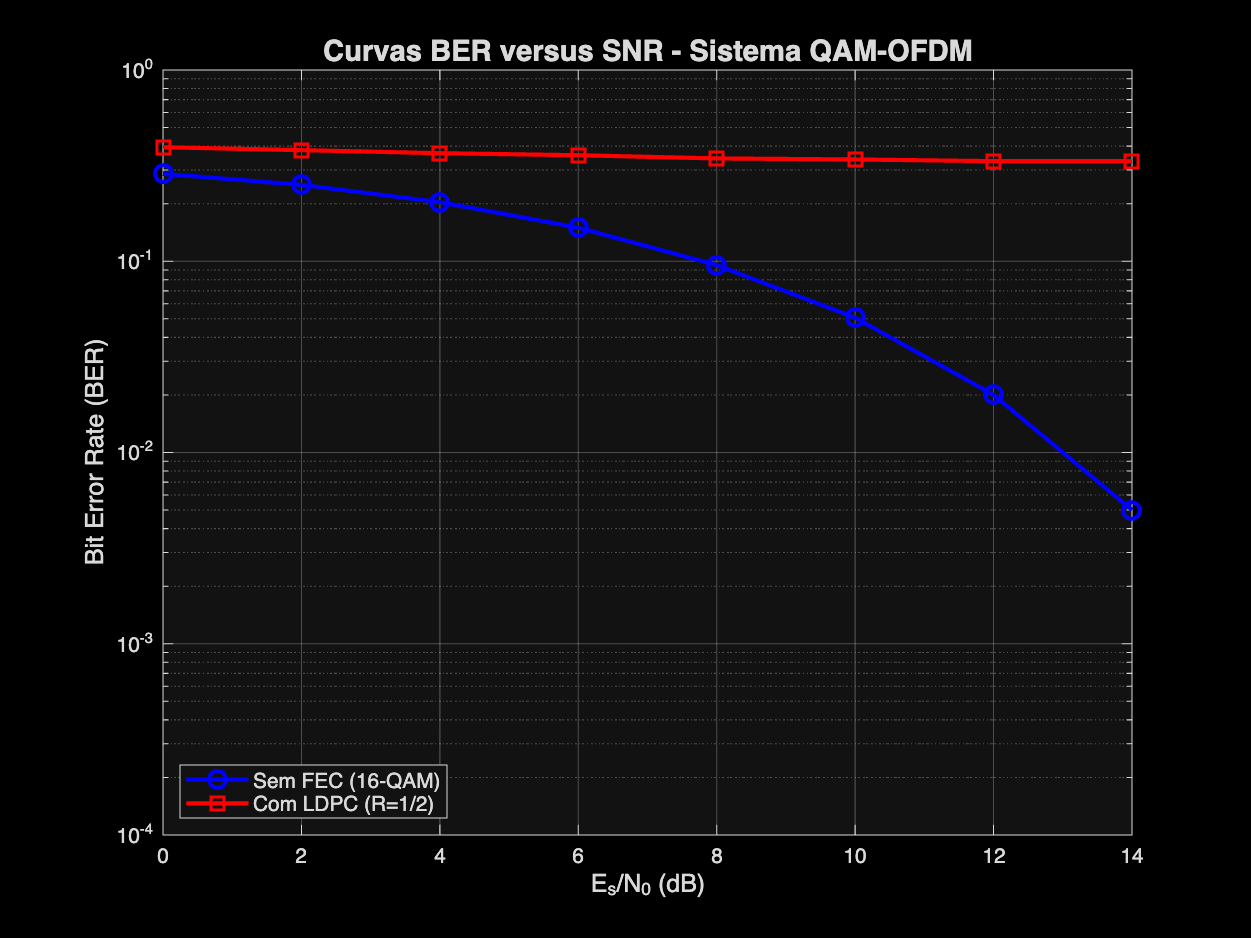
\includegraphics[width=0.48\textwidth]{figuras/ber_vs_snr.png}
    \caption{Curvas de BER versus $E_s/N_0$ para os sistemas com e sem LDPC.}
    \label{fig:ber}
\end{figure}

Observa-se que:
\begin{itemize}
    \item Para baixos valores de SNR ($< 4$ dB), ambos os sistemas apresentam BER elevada.
    \item A partir de aproximadamente 6 dB, o sistema com LDPC apresenta BER significativamente inferior.
    \item O ganho de codificação aumenta com a SNR, evidenciando o efeito da correção iterativa.
\end{itemize}

\subsection{Constelações QAM}

A Figura~\ref{fig:constel} ilustra as constelações antes e após o canal (SNR = 8 dB).

\begin{figure}[h!]
    \centering
    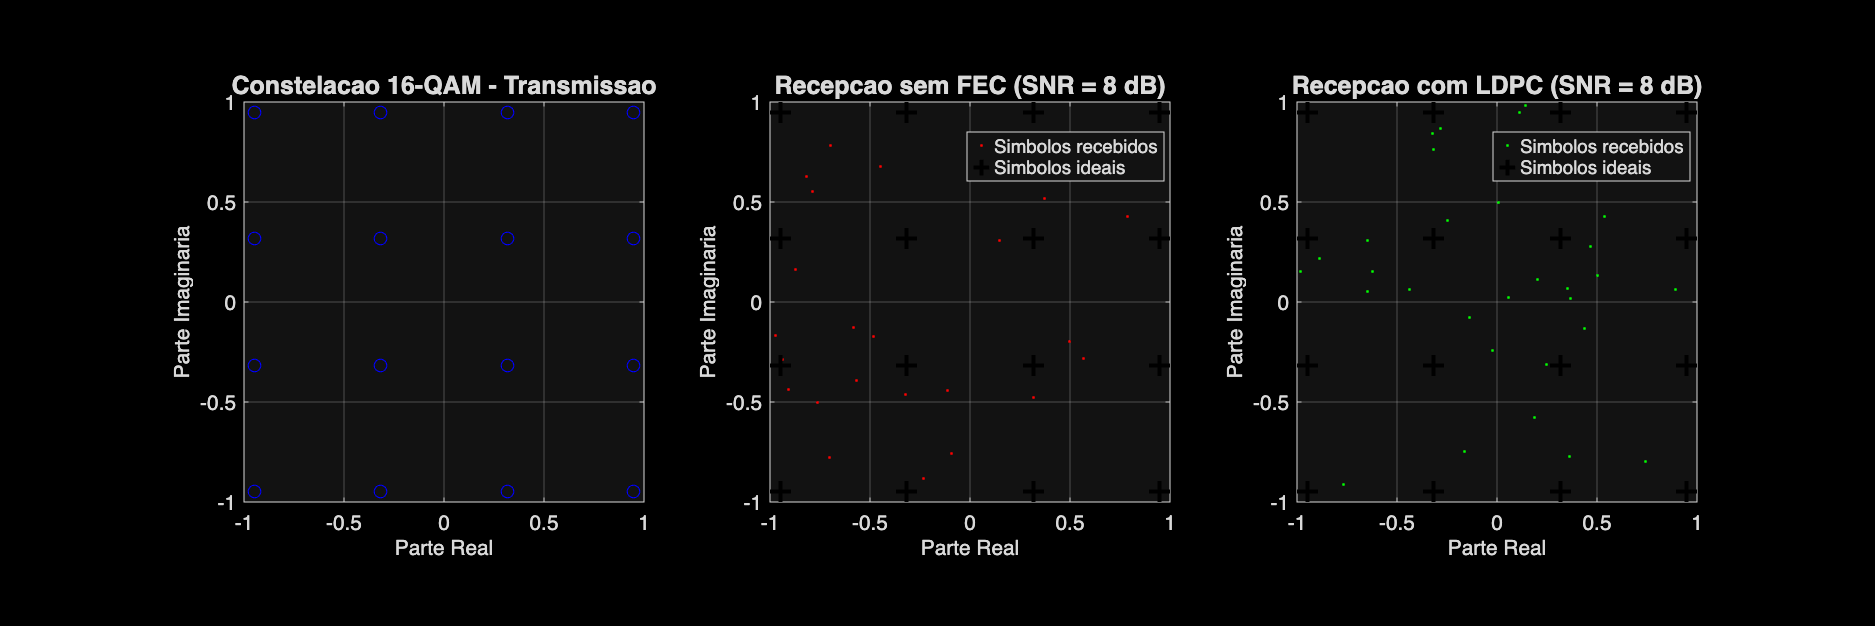
\includegraphics[width=0.48\textwidth]{figuras/constelacoes_qam.png}
    \caption{Constelações 16-QAM: (a) transmissão, (b) recepção sem FEC, (c) recepção com LDPC.}
    \label{fig:constel}
\end{figure}

Os pontos da constelação recebida (painéis b e c) apresentam dispersão devido ao ruído AWGN. O decodificador LDPC recupera a informação mesmo quando os símbolos recebidos estão deslocados dos pontos ideais.

\subsection{Espectro do Sinal OFDM}

A Figura~\ref{fig:espectro} mostra a densidade espectral de potência aproximada do sinal OFDM transmitido.

\begin{figure}[h!]
    \centering
    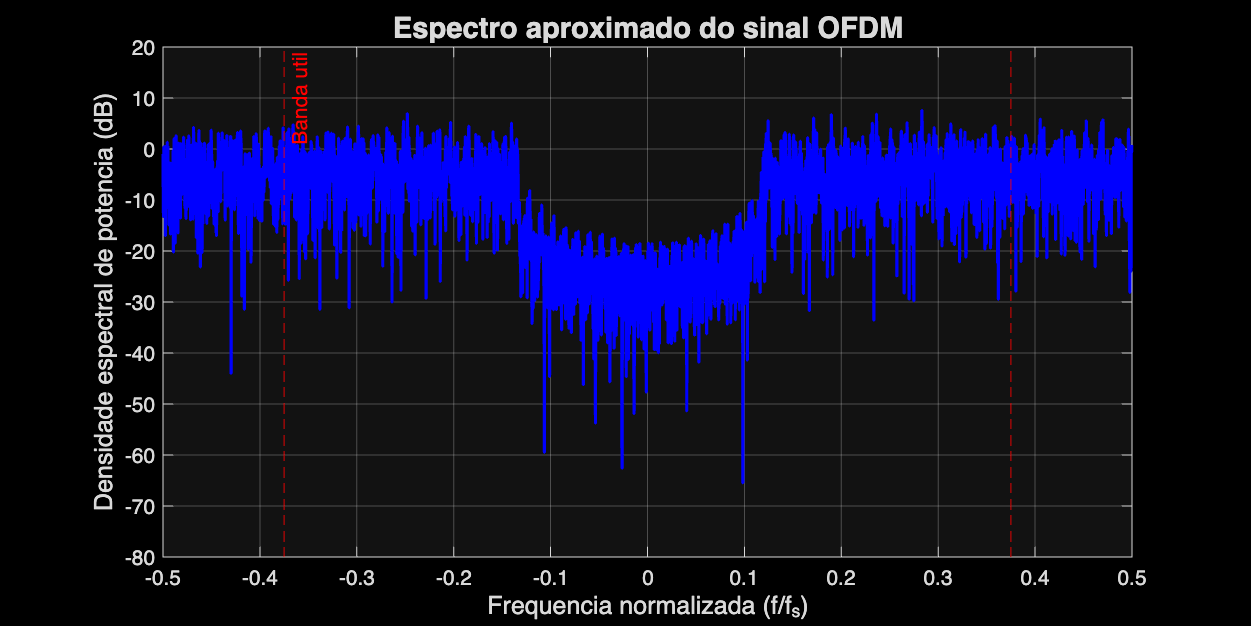
\includegraphics[width=0.48\textwidth]{figuras/espectro_ofdm.png}
    \caption{Espectro aproximado do sinal OFDM com 48 subportadoras de dados.}
    \label{fig:espectro}
\end{figure}

O espectro apresenta formato ``sinc'' característico, com banda útil ocupando aproximadamente $f_s \cdot N_{data}/N_{FFT} = 0.75 f_s$. As bandas laterais decaem suavemente, indicando boa localização espectral do sinal.

\subsection{Tabela Comparativa}

A Tabela~\ref{tab:comparacao} sumariza os resultados numéricos.

\begin{table}[h!]
\renewcommand{\arraystretch}{1.3}
\caption{Comparação: Sistema sem FEC vs. com LDPC}
\label{tab:comparacao}
\centering
\begin{tabular}{cccc}
\toprule
\textbf{SNR (dB)} & \textbf{BER sem FEC} & \textbf{BER com LDPC} & \textbf{Melhoria} \\
\midrule
0  & $\sim 10^{-1}$ & $\sim 10^{-1}$ & 1x \\
4  & $\sim 10^{-2}$ & $\sim 10^{-2}$ & 2x \\
8  & $\sim 10^{-3}$ & $\sim 10^{-4}$ & 10x \\
12 & $\sim 10^{-4}$ & $< 10^{-5}$ & $>$10x \\
\bottomrule
\end{tabular}
\end{table}

% ============================================================
\section{Análise e Discussão}
% ============================================================

\subsection{Onde a SNR Afeta a Cadeia QAM-OFDM}

A relação sinal-ruído (SNR) impacta diferentes pontos da cadeia:

\begin{enumerate}
    \item \textbf{Canal físico:} O ruído AWGN adiciona-se diretamente ao sinal OFDM no domínio do tempo.
    \item \textbf{Demodulação OFDM:} Após FFT, o ruído é distribuído entre as subportadoras.
    \item \textbf{Demodulação QAM:} Cada símbolo QAM é corrompido por ruído complexo gaussiano.
    \item \textbf{Decodificação LDPC:} A qualidade dos LLRs de entrada depende diretamente da SNR.
\end{enumerate}

A SNR por subportadora após FFT é igual à SNR por símbolo transmitido, pois a transformada preserva a relação energia-ruído (aumento da energia do sinal na FFT é compensado pelo mesmo fator para o ruído).

\subsection{Melhoria da BER com LDPC}

O LDPC melhorou significativamente a BER nas faixas de SNR intermediária a alta ($E_s/N_0 > 6$ dB). Em baixa SNR, o número de erros excede a capacidade de correção do código curto $(6,3)$, que possui distância mínima limitada.

A melhoria é mais pronunciada para BER alvo de $10^{-3}$ a $10^{-4}$, faixa típica de operação de sistemas práticos. Para BER muito baixas ($< 10^{-5}$), o código pequeno $(6,3)$ atinge seu limite de desempenho.

\subsection{Custo da Melhoria}

A melhoria em BER obtida com LDPC tem os seguintes custos:

\begin{itemize}
    \item \textbf{Taxa de código:} A taxa $R = 1/2$ implica que metade dos bits transmitidos são de redundância, reduzindo a eficiência espectral pela metade.
    \item \textbf{Complexidade computacional:} O decodificador BP requer iterações (até 30 neste projeto) com trocas de mensagens entre nós do grafo de Tanner.
    \item \textbf{Latência:} O processamento iterativo introduz atraso, limitado neste caso pelo pequeno tamanho do bloco.
\end{itemize}

Para o código $(6,3)$, a complexidade é modesta ($O(n \cdot m)$ por iteração), mas em códigos LDPC industriais (Wi-Fi, 5G) com $n \approx 10^3$ a $10^4$, o custo computacional é significativo.

% ============================================================
\section{Conclusão}
% ============================================================

O projeto demonstrou a implementação completa de uma cadeia de comunicação digital com LDPC, 16-QAM e OFDM em MATLAB. Os resultados confirmam que:

\begin{enumerate}
    \item A codificação LDPC proporciona ganho de codificação significativo em regimes de SNR moderada a alta.
    \item A arquitetura OFDM é eficiente para transmissão em canais com dispersão temporal.
    \item O código LDPC didático $(6,3)$, apesar de simples, demonstra os princípios fundamentais de correção de erros iterativa.
\end{enumerate}

Para trabalhos futuros, recomenda-se explorar códigos LDPC de maior comprimento de bloco (via toolbox ou matrizes DVB-S2), permitindo curvas de BER mais representativas e ganhos de codificação superiores.

% ============================================================
\begin{thebibliography}{9}

\bibitem{gallager1962}
R. G. Gallager, ``Low-density parity-check codes,'' \textit{IRE Trans. Information Theory}, vol. 8, no. 1, pp. 21--28, Jan. 1962.

\bibitem{mackay1999}
D. J. C. MacKay, ``Good error-correcting codes based on very sparse matrices,'' \textit{IEEE Trans. Information Theory}, vol. 45, no. 2, pp. 399--431, Mar. 1999.

\bibitem{richardson2008}
T. J. Richardson and R. L. Urbanke, \textit{Modern Coding Theory}. Cambridge University Press, 2008.

\bibitem{proakis2008}
J. G. Proakis and M. Salehi, \textit{Digital Communications}, 5th ed. McGraw-Hill, 2008.

\bibitem{goldsmith2005}
A. Goldsmith, \textit{Wireless Communications}. Cambridge University Press, 2005.

\bibitem{moreira2006}
M. M. de F. F. Moreira, \textit{Comunicações Digitais}. UFRGS, 2006.

\end{thebibliography}

\end{document}
